\documentclass[11pt,a4paper]{article}

\usepackage[utf8]{inputenc}
\usepackage[T1]{fontenc}
\usepackage[margin=2cm]{geometry}
\usepackage{lmodern}
\usepackage{xcolor}
\usepackage{booktabs}
\usepackage{tabularx}
\usepackage{enumitem}
\usepackage{amsmath}
\usepackage{tikz}
\usetikzlibrary{arrows.meta,positioning,fit}
\usepackage[hidelinks]{hyperref}
\usepackage{fancyhdr}

\definecolor{ocpgreen}{HTML}{007A5E}
\definecolor{lightgreen}{HTML}{EAF5F1}
\definecolor{darkgray}{HTML}{374151}
\newcolumntype{Y}{>{\raggedright\arraybackslash}X}
\newcolumntype{L}[1]{>{\raggedright\arraybackslash}p{#1}}
\newcommand{\code}[1]{\texttt{\detokenize{#1}}}
\newcommand{\filepath}[1]{\nolinkurl{#1}}

\pagestyle{fancy}
\fancyhf{}
\lhead{SLURRY\_FREE\_ACID industrial deployment}
\rhead{Ikram Benfellah}
\cfoot{\thepage}
\setlength{\headheight}{14pt}
\setlist[itemize]{leftmargin=1.3em,itemsep=2pt,topsep=3pt}
\setlist[enumerate]{leftmargin=1.5em,itemsep=2pt,topsep=3pt}
\setlength{\parindent}{0pt}
\setlength{\parskip}{5pt}

\title{\textbf{Industrial Deployment Prototype for\\SLURRY\_FREE\_ACID Estimation}}
\author{Ikram Benfellah}
\date{1 September 2026}

\begin{document}
\maketitle

\begin{center}
\colorbox{lightgreen}{\parbox{0.91\textwidth}{
\textbf{Purpose.} I prepared the first isolated deployment prototype that connects the selected Python model to an OPC UA data source. The current system is a laboratory test using CSV replay.
}}
\end{center}

\section{Architecture and responsibility boundary}

\begin{center}
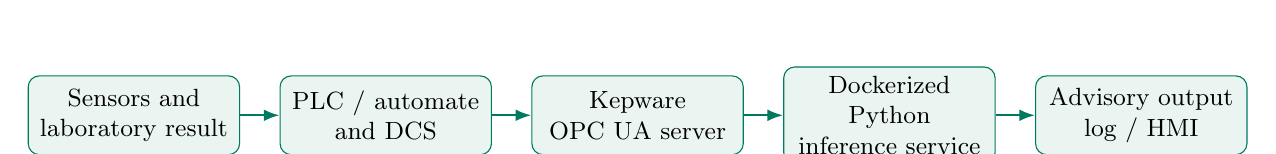
\begin{tikzpicture}[
  node distance=5mm and 5mm,
  box/.style={draw=ocpgreen,rounded corners,fill=lightgreen,minimum height=10mm,
              text width=2.45cm,align=center,font=\small},
  arrow/.style={-{Latex[length=2mm]},thick,draw=ocpgreen}
]
\node[box] (physical) {Sensors and\\laboratory result};
\node[box,right=of physical] (plc) {PLC / automate\\and DCS};
\node[box,right=of plc] (kep) {Kepware\\OPC UA server};
\node[box,right=of kep] (docker) {Dockerized Python\\inference service};
\node[box,right=of docker] (output) {Advisory output\\log / HMI};
\draw[arrow] (physical)--(plc);
\draw[arrow] (plc)--(kep);
\draw[arrow] (kep)--(docker);
\draw[arrow] (docker)--(output);
\end{tikzpicture}
\end{center}

\begin{tabularx}{\textwidth}{@{}L{2.6cm}YY@{}}
\toprule
\textbf{Component} & \textbf{Role} & \textbf{Safety boundary} \\
\midrule
Sensors / actuators & Measure the process; valves, pumps and motors act on it. & The ML service does not directly access actuator commands. \\
PLC / DCS & Deterministic control, interlocks, alarms and operator supervision. & Plant safety remains independent of model availability. \\
Kepware & Translates controller-specific protocols and exposes approved tags through OPC UA. & It is a communication gateway, not a prediction model. \\
Docker service & Validates measurements, keeps recent history, builds model features and runs inference. & Advisory only; no setpoint, interlock, valve or pump control. \\
Operator / HMI & Displays and interprets the advisory result. & The operator remains the decision-maker. \\
\bottomrule
\end{tabularx}

\section{What I implemented}

The work is organized under \code{deployment/} so that deployment logic is separated from the research notebooks.

\begin{tabularx}{\textwidth}{@{}L{3.2cm}Y Y@{}}
\toprule
\textbf{Element} & \textbf{Implementation} & \textbf{Purpose} \\
\midrule
OPC UA simulator & A separate Python container replays the historical one-minute CSV and exposes configured OPC nodes. & Test the client/server boundary without connecting to the plant. \\
Inference service & A second Python container subscribes to a commit-sequence tag, reads coherent snapshots and loads the saved model artifacts. & Reproduce the intended live inference flow. \\
Docker Compose & Creates both containers on a private Docker network; the simulator exposes port 4840. & Reproducible and isolated Stage~1 environment on Windows/Docker Desktop. \\
Tag mapping & \code{config/opc_tags.yaml} maps research variable names to OPC Node IDs, units and required-tag metadata. & Avoid hard-coded plant addresses; real Node IDs can be substituted later. \\
Service policy & \code{config/service.yaml} centralizes mode, cadence, buffer, quality and output settings. & Keep operational choices visible and auditable. \\
Data-quality shield & Allows isolated missing cells through the trained imputation pipeline, but rejects excessive missingness, bad/uncertain OPC quality, invalid chronology, excessive gaps and configured impossible values. & Continue safely through ordinary missing cells without hiding serious data loss. \\
Runtime outputs & Health status, complete JSONL prediction history and one readable latest-prediction JSON file. & Monitoring, audit and simple human inspection. \\
PowerShell scripts & Start, stop and readable status commands. & Make the laboratory prototype easy to operate. \\
\bottomrule
\end{tabularx}

\subsection*{Model operating modes}

\begin{itemize}
  \item \textbf{Target-free mode (current default):} process measurements only $\rightarrow$ estimate of the current \code{SLURRY_FREE_ACID}. The deployed candidate is the selected five-cluster Ridge virtual sensor. This is a soft sensor, not a ten-minute forecast.
  \item \textbf{Target-anchored mode:} process measurements plus a sufficiently recent free-acid value $y_t$ $\rightarrow$ predicted change $\widehat{\Delta y}_{t,h}$, reconstructed as
  \[
     \widehat y_{t+h}=y_t+\widehat{\Delta y}_{t,h}.
  \]
  Because free acid is currently a manual laboratory result, this mode requires a reliable laboratory-result timestamp and freshness policy.
\end{itemize}

\section{Streaming, warm-up and output logic}

\begin{enumerate}
  \item The simulator updates all process tags, the source timestamp, then a sequence tag as the final commit marker.
  \item The inference client subscribes to the sequence tag rather than polling continuously.
  \item For each notification, the sequence is read before and after the process values. The snapshot is accepted only when both reads agree; this prevents mixing two CSV rows.
  \item The data-quality shield validates the snapshot.
  \item Accepted rows enter a chronological rolling buffer. The model then recreates the feature order and preprocessing used during training.
  \item The prediction and its context are written to audit files. Advisory OPC writes remain disabled by default.
\end{enumerate}

\textbf{Why 31 rows are required.} The feature pipeline has a 30-minute maximum lookback. It therefore needs 30 historical minutes plus the current row:
\[
\text{minimum rows}=30+1=31.
\]
The service reports \code{WARMING_UP} while this initial history is collected. An isolated missing cell does not restart the buffer: Notebook~02's train-fitted imputer and missingness indicators handle it, and the output reports \code{IMPUTED}. A real timestamp gap, reconnect, bad OPC quality or more than 25\% of required inputs missing together still blocks inference. In production, the initial delay should be avoided by backfilling the last 30 minutes from the plant historian and, if approved, restoring a validated persistent local buffer.

\begin{tabularx}{\textwidth}{@{}L{3.4cm}Y@{}}
\toprule
\textbf{Output} & \textbf{Meaning} \\
\midrule
\filepath{runtime/health.json} & Machine-readable state such as STARTING, CONNECTED, WARMING\_UP, RUNNING, DATA\_ERROR or DISCONNECTED, with an explicit reason. \\
\filepath{runtime/latest_prediction.json} & One formatted latest successful prediction for inspection. \\
\filepath{runtime/predictions.jsonl} & Append-only prediction history for audit and later comparison with laboratory results. \\
\filepath{scripts/status_stage1.ps1} & Short human-readable status: collected/required rows, reason for an error and latest prediction. \\
\bottomrule
\end{tabularx}

\section{Stage 1 validation and corrections}

The complete laboratory path was executed: Docker images were built, the OPC UA server started, the inference client connected and subscribed, model artifacts loaded, and prediction records were generated. The following engineering issues were identified and corrected during testing.

\begin{tabularx}{\textwidth}{@{}L{3.4cm}Y Y@{}}
\toprule
\textbf{Observed issue} & \textbf{Cause} & \textbf{Correction} \\
\midrule
Docker Hub TLS timeout & Temporary registry/network timeout while downloading the base image. & Added explicit pull checking, retry logic and a clear network diagnostic; TLS verification was not disabled. \\
PowerShell Compose call failed & Docker arguments were not forwarded as an array. & Corrected the wrapper to pass all arguments and check exit codes. \\
LightGBM could not load & Linux image lacked the OpenMP runtime. & Installed \code{libgomp1} and added a build-time import check. \\
Client initially read the last replayed row & The simulator continued while the inference container had previously failed. & Restarted the complete laboratory environment from a clean replay state. \\
Duplicate/non-monotonic timestamps & Replay at 0.10 s was faster than the OPC publication/reading cycle. & Changed replay to 1.00 s, subscription to 100 ms, added coherent sequence-guarded reads and ignored already processed sequence values. \\
Prediction file absent during warm-up & It was created only after the first prediction. & Create the history file at startup and expose a separate readable latest-prediction file. \\
Unreadable protocol logs & OPC library INFO messages included full protocol packets. & Reduced library logging and added a concise status script. \\
\bottomrule
\end{tabularx}

\textbf{Current interpretation of quality status.} \code{GOOD} means no input required imputation. \code{IMPUTED} means prediction continued and lists the missing sensors handled by the trained pipeline. \code{DATA_ERROR} is reserved for a serious input problem such as excessive simultaneous missingness, bad OPC quality or invalid chronology; it is not necessarily a container failure.

\section{Current limits and next steps}

\textbf{Already demonstrated}
\begin{itemize}
  \item isolated two-container OPC UA inference path;
  \item configuration-based tag mapping and model loading;
  \item subscription, reconnect, chronological buffering and warm-up behavior;
  \item explicit quality rejection and auditable prediction output;
  \item advisory-only safety boundary.
\end{itemize}

\textbf{Still required before plant shadow mode}
\begin{enumerate}
  \item Confirm the DCS/PLC vendors, Kepware version, OPC UA endpoint, security policy, certificates and firewall route.
  \item Replace placeholder Node IDs; confirm engineering units, physical limits and OPC quality semantics for every tag.
  \item Add historian backfill/persistent-buffer recovery so a restart does not require 31 new live minutes.
\end{enumerate}

\begin{center}
\colorbox{lightgreen}{\parbox{0.91\textwidth}{
\textbf{Conclusion.} Stage~1 proves that the research model can be packaged and connected through an OPC UA boundary in an isolated environment. It does not yet prove production accuracy or authorize operational intervention. The next technical milestone is a secured laboratory Kepware connection, followed by read-only shadow validation using correctly timestamped plant and laboratory data.
}}
\end{center}

\end{document}
